\section{Introduction to bands}

% Le plus gros du morceau arrive lorsque l'on s'intéresse à la représentation
% réelle du document que l'on souhaite imprimer. Dans un premier temps,
% l'étude de la représentation sera faite (dans cette section même) pour
% embrayer ensuite sur les différents algorithmes de compression des
% << bandes >>.
%
The largest piece of the puzzle is the real representation of the document you want to print.
For the first time, the study of this format has been done (in this very section).  Following
is a discussion of the different ``band'' compression algorithms.

\subsection{From document to bitmap}

\noindent\textit{\underline{Note : }
Since the present study was only done on a black and white printer, this will
be the only type of printing discussed.}

\medskip
In contrast to languages like \emph{PostScript}, that are vector based
languages, QPDL is a language that describes images dot by dot.

To print a document it is therefore necessary to convert it to an image
where each bit corresponds to a dot on the page.  The format closest to
that understood by the printer is PBM\footnote{Portable BitMap}.

To review, the PBM format describes an image bit by bit without compression. A set bit corresponds to a black dot and a zero bit corresponds to a white dot. Adjacent bits represent lines and the byte
which follows the end of a line starts the beginning of the next.  This continues until the
end of the file.

\subsection{From image to bands}

Once the document is converted into an image, it is necessary to cut it
into bands.  The bands represent a fixed number of lines of dots: one band
represents exactly \emph{128 lines} (that's $0x80$).

\subsection{An image in columns}

In contrast to a PBM image which describes an image line by line, the printer expects the
image in bands that represent the image \emph{column by column}. In fact, the first
byte represents the first byte of the first line, the second byte represents the first byte of the second line, \ldots. Then the 129\raise{th} byte represents the second byte of the first line.

Figure \ref{fig:bande} represents this treatment.

\begin{figure}[ht]
\centering
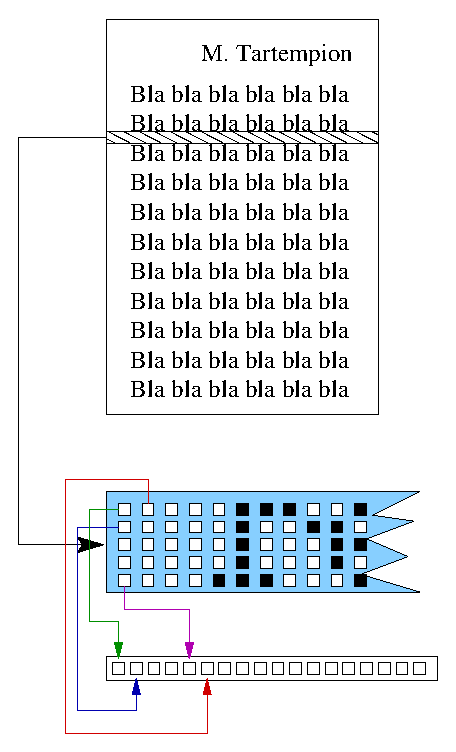
\includegraphics{Images/bande.eps}
\caption{From a document to rearranged data}
\label{fig:bande}
\end{figure}

\subsection{Bit inversion}
Whereas in a PBM file a set bit corresponds to a black bit, for the
printer is is the reverse.
It is thus essential to apply the \emph{NOT} operator to each byte in the band.

\section{Band header}

The band header gives invaluable directions on how to convert
the band and recreate the document. As table 
\ref{tab:entete_bande} shows.

\begin{table}[!ht]
\centering
\begin{tabular}{| c | c | c |}
\hline
\textbf{Address} & \textbf{Description} & \textbf{Type} \\
\hline
\hline
0x0 & Fixed value $0xC$ & Byte \\
0x1 & Band number & Byte \\
0x2 & Width of band & 16-Bits BE \\
0x4 & Height of band & 16-Bits BE \\
0x6 & Compression version $0x11$ (?) & Byte \\
0x7 & Length of following data & 32-Bits BE \\
\hline
\end{tabular}
\caption{Band Header}
\label{tab:entete_bande}
\end{table}

\section{Band compression}
To reduce the quantity of data transmitted to the printer, the band data is compressed. There
appear to be several compression versions. The following description covers the
version most often seen, version \textsc{$0x11$}.

\subsection{Compressed data header}
The  information required to decompress the data is
provided in the header.  A description of which is found
in table\ref{tab:entete_compression}.
In contrast to the other headers, this header can be written
without worrying about whether the machine is 
\emph{little-endian} or \emph{big-endian}. Indeed, when the header 
signature is written ($0x9ABCDEF$), the printer will autodetect 
the endianness of the following 
data. It is thus enough to write the data without any special conversion.

\begin{table}[!ht]
\centering
\begin{tabular}{| c | c | c |}
\hline
\textbf{Adresse} & \textbf{Description} & \textbf{Type} \\
\hline
\hline
0x0 & Fixed value $0x9ABCDEF$ & 32-Bits \\
0x4 & Raw data length ($ \leq 128$) & 32-Bits \\
0x8 & Pointer table & 64 16-Bit entries \\
0x88 & Raw data & Variable \\
Variable & Compressed data & Variable \\
\hline
\end{tabular}
\caption{Compressed data header}
\label{tab:entete_compression}
\end{table}

The significance of the various entries follows.

\subsection{The Compression Algorithm}
The compression algorithm aims to reduce sequences of similar bytes.
With this aim, a table of $64$ \emph{offsets} is initialized, and the beginning of the uncompressed
raw data is copied.
Then, for each entry in the table, one compares the following data to be compressed with previous uncompressed data using the table entry as a negative offset from the current position.
The index of the table entry that provides the longest sequence is kept and its index
and the length of the sequence is output.
If, however, no matching sequence can be found, the following data will be written out
uncompressed until a sequence using one of the offsets in the table can be found.

\subsection{An example of compression}
The study of a concrete example permits a better understanding.
Here's a table with 4 entries:

\begin{exemple}
Table = \{-1; -3; -4; -5\}
\end{exemple}

with initial raw data as follows:
\begin{exemple}
01 04 03 06 08 0F 0F 0F 0F 04 02 05 08 01 06 03 06 01 06
\end{exemple}

The following data is to be compressed:
\begin{exemple}
0F 0F 01 04 03 06 0F 01 04 05 06 0F 01 04 05 06 0F 0F 0F 0F 0F
\end{exemple}

To find the best sequence, it is necessary to try each pointer. Each pointer is 
tried relative to the current position.
Taking the first pointer, the comparison is done between 06 and 0F
The comparison stops there. It is noticed that for the three other pointers,
no matching sequence is found. Therefore $0F$ will be written out uncompressed.

For the second character, the first pointer is valid for a sequence of length
one; and that's the only pointer that matches a sequence.  Unfortunately, if
the length of a sequence is \emph{less than 3} compression is not useful.
It is therefore preferable to output the data uncompressed.

This is the same for the four next characters.  With the seventh character,
the fourth pointer gives us a sequence of three characters.

The next character is written out uncompressed.  Following that, the fourth
pointer matches a sequence of length seven.

Finally, to finish, the first pointer matches a sequence of four bytes.
\medskip

To review, the compressed data may be represented as follows:
\begin{exemple}
Uncompressed data : 0F 0F 01 04 03 06 \\
Pointer 4, length = 3 \\
Uncompressed data : 05 \\
Pointer 4, length = 7 \\
Pointer 1, length = 4
\end{exemple}


\subsection{Compression coding}
As we saw above, a table of pointers is stored in the header.
Each entry is the absolute value of a displacement.
So, to represent a displacement of $-1$, the entry will be $1$.
Uncompressed data follows the header.
The amount of this uncompressed data is the maximum of $128$ and the largest pointer value (in absolute value). So, if the largest pointer value is greater then $128$, only $128$ bytes
of uncompressed data follows.
Finally, this quantity of data is copied out of the header into the start of
the uncompressed data.

What follows is the compressed data.
If a sequence of data can be compressed, \emph{bit 7} of the first byte is
set and the remaining seven bits encode the least significant bits of the
\emph{sequence length}.  Finally, bits $6$ and $7$ of the second byte encode
bits seven and eight of the \emph{sequence length} whilst the other bits encode
an index into the pointer table.
It should be noted that three must be \emph{subracted} from the sequence length
before being encoded and this explains why it is not possible to represent
sequences of less than three bytes.

On the other hand, if a sequence of data cannot be compressed,
% 128 surely?
this data is cut into sequences of 64 bytes (in case it's longer)
and the first byte encodes the length minus one of the uncompressed data that follows.

A small summary is given in figure \ref{fig:code_comp}.
\begin{figure}[!ht]
\centering
\begin{verbatim}
unsigned short length, ptr;

if (byte1 & 0x80) {
    length = (byte1 & 0x7F) + ((byte2 & 0xC0) << 1) + 3;
    ptr = byte2 & 0x3F;
} else {
    length = byte1 + 1;
}
\end{verbatim}
\caption{Sequence encoding}
\label{fig:code_comp}
\end{figure}

To repeat the previous example, here's how it would be compressed:
\begin{exemple}
05 0F 0F 01 04 03 06 80 04 00 05 84 04 81 01
\end{exemple}

That's six bytes shorter than the uncompressed data.

\section{Checksum}
To be able to detect data corruption during transit, a
checksum is placed at the end of the compressed data (it should be noted
that the length of this checksum is included in the 
data length indicated in the band header).
This sum is coded
as 32-bits big-endian and is the simple sum of the bytes between
the band header and the checksum.

